\chapter{System architecture}
The library is based on the client-server architectural pattern and his functionalities are indeed split in two distinct modules: 
\begin{itemize}
	\item \textit{Client module} - Provides the main methods to connect and communicate with a game server. In particular allows the client side developer to create rooms (that will be hosted on the server) and to perform operations on them (e.g join, leave, message...).
	\item \textit{Server module} - Internally implements the logic to handle client connections and allows the developer to run a gameserver and define new type of rooms. It also contains all the logic to handle matchmaking requests.
\end{itemize}

Client and server modules are not fully separated; they share some common concepts like communication protocol and data serialization utilities to parse data received and sent through the network. All these are grouped in a common packages used by both client and server.

The most important concept that client and server share is anyway the concept of room that is described in detail in the next section. 

\section{Room}


\begin{figure}[H]
	\centering
	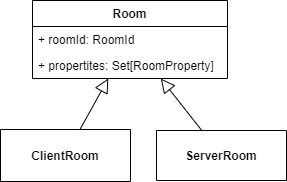
\includegraphics[scale=0.7]{images/3-architecture/room-class-3.png}
	\caption{Room class diagram}
	\label{fig:room_classes}
\end{figure}


At the most abstract level, a room is an entity with a unique id and some shared properties that 'describe' the room (figure \ref{fig:room_classes}). This fields are accessible both on the client and the server. Then each module extends his own concept of room.

\bigskip
\textit{ServerRoom}
\\
The server room is the one that will be used by the server side developer. It provides methods to communicate and interact with clients who are connected to ther room. Its behavior can be defined by the developer according to the application logic he wants to implement.

\bigskip
\textit{ClientRoom}
\\
This is, on the other hand, the room that a client side developer will use. This component is meant to provide an interface towards the server side room so that the developer can both send and receive messages from it.

\section{Server architecture} \label{sec:server_arch}
The main components of the server side architecture are visible in figure \ref{fig:server_classes}. 

\begin{figure}[H]
	\centering
	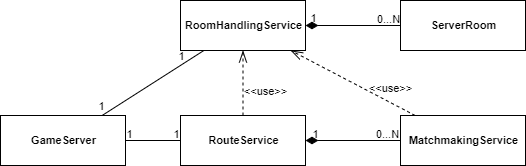
\includegraphics[scale=0.7]{images/3-architecture/server-architecture.png}
	\caption{Server architecture}
	\label{fig:server_classes}
\end{figure}

\bigskip
\textit{GameServer}
\\
The GameServer is the main component of the architecture. It is the one that listen and handle client connections and is also the starting point from where all the other components are created.

A developer will mostly use the server module of the library working with the interface that this component exposes.

As shown in figure \ref{fig:server_classes} it is connected with two other classes that are the RouteService and the RoomHandlingService.

\bigskip
\textit{RoomHandlingService}
\\
As the name suggests, the RoomHandler is the component used to manage rooms. It is meant to: 
\begin{itemize}
	\item Keep track of which rooms are currently active in the system providing a way to interact with them (e.g create new ones or delete existing)
	\item Provide a way to define new type of rooms that, upon a specific client requests, will be created.
\end{itemize}

\bigskip
\textit{RouteService}
\\
Defines the routes that the clients should use to interact with the server and implements all the handlers associated with them. A client request received by the gameserver is indeed served by this component. 

Client requests can basically be split in two types:
\begin{itemize}
	\item requests concerning rooms (e.g connect to a room or retreive available rooms...)
	\item requests concerning matchamking (e.g join a matchmaking queue)
\end{itemize}
This component uses a RoomHandler to manage the first type and a list of MatchamkingServices (one for each type of room defined by the user) for the second type. 

\bigskip
\textit{MatchmakingService}
\\
The MatchmakingService is the component that implement the matchmaking logic for a given type of room (i.e. adding clients to a queue and eventually create groups according to some information on those clients). It also needs to use a RoomHandler since, when the a group of client is formed, a room where this clients will connect must be created.



\section{Client Architecture}

RS

\section{Client-Server Interaction}
The requirements analysis led to the definition of three types of interaction between client and server:
\begin{enumerate}
	\item Client to GameServer \\
	This interaction takes place in those situations where the client makes a request to the server and waits for a specific response: for example getting the list of all joinable rooms. We decided to handle this kind of requests defining a REST protocol as shown in table
	 \ref{table:server_routes}.
	\begin{table}[]
		\begin{tabular}{p{2cm}p{4cm}p{2cm}p{5.5cm}}
			\textbf{Http Method} & \textbf{Path}	  & \textbf{Payload}  & \textbf{Result}                                                            		\\\\
			GET                  & /rooms             & filters           & get all the rooms that match the filters in the payload                        	\\\\
			GET                  & /rooms/:type       & filters           & get all the rooms with the given type (filtered by filters in the payload)     	\\\\
			GET                  & /rooms/:type/:id   & empty             & get the room with the given id searching among rooms of the given type         	\\\\
			POST                 & /rooms/:type       & options           & create a room of the given type with the option passed in the payload          	\\\\
			GET                  & /connection/:id    & websocket request & open a web socket connection with the room that has the given id               	\\\\
			GET                  & /matchmaking/:type & websocket request & open a web socket with the matchmaking service relative to the given room type 	\\\\
		\end{tabular}
		\caption{\label{table:server_routes} \textit{Server REST protocol for request-response interaction}}
	\end{table}
	\item  Client to Room \\
	In this case we are in a situation where a client wants to establish a connection with a given a room to both send and receive messages from it. The request-response pattern doesn't work here because now the communication channel must be full-duplex: the server can send data to the client even without a specific client request (for example if the room broadcasts a message to all connected clients).
	
	The chosen solution here is the webosckets protocol since it provides the exact described behavior. Specifically, when a client wants to interact with a room, a websocket between that client and the server is created; the messages that the client sends through the socket are redirected to the room and the messages that the room wants to send to that client are forwarded through the socket. 
	
	Another consideration to make here is that clients can receive and send different types of messages through the socket: first of all they need to send a join message to notify the room that they want to enter; then they may want to send generic messages to that room (e.g. actions that affect the current game state) and eventually they'll want to leave the room, and so on \dots
	In order to identify this different kind of messages we decided to define a communication protocol that is used for messages in the websocket.
	
	
	\item Client to Matchmaking \\
	The last type of interaction is the one that takes place when a client wants to join the matchmaking queue for a given type of room. In this case the client asks the server to be added to the queue and waits to be grouped with other clients. We have decided to use websockets here too since when the client sends the request, the server response is not immediate. The communication must be kept open until the matchmaking service doesn't create the group of client to start the match. Only then the server can respond to the client with a message that contains the information to join the room that will host the game.
\end{enumerate}









